\documentclass[tikz,border=3.14mm]{standalone}
\begin{document}
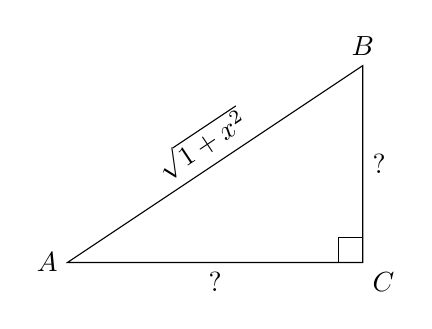
\begin{tikzpicture}[scale=1.25]
\draw  (-1.5,-1) coordinate [label=left:$A$] (A) -- 
  node[midway,above,sloped] {$\sqrt{1+x^2}$} 
  (1.5,1) coordinate [label=above:$B$] (B) --
  node[right] {?} 
  (1.5,-1)coordinate [label=below right:$C$] (C) -- 
  node[below] {?} cycle;
\draw ([xshift=-0.25cm]C) |- ([yshift=0.25cm]C);
\end{tikzpicture}
\end{document}